\documentclass[12pt,a4paper]{article}
\synctex=1
\usepackage[utf8]{inputenc}
\usepackage[margin=1cm]{geometry}
\usepackage{graphicx}
%\usepackage{verbatim}
\usepackage{amsmath}
\usepackage{amsfonts}
\usepackage{amssymb}
\usepackage{listings}
\usepackage{enumitem}
\usepackage{textcomp}
\usepackage{courier}
\usepackage{libertine}
\usepackage{pgfornament}
\usepackage{eso-pic}
\usepackage[hangul]{kotex}
\linespread{1.3}

\title{
	\centering
	\pgfornament[width=12cm,color=teal]{84}\\
	\vspace{1cm}
	\fontsize{50}{50} \selectfont {정보통신 수학 및 실습\\Lab assignment}\\
		\pgfornament[width=12cm,color=teal]{88}\\
	\vfill}
\author{
	\LARGE
	\begin{tabular}{rl}
		\hline
		학번 : & 2016110056\\ 
		학과 : & 불교학부 \\
		이름 : & 박승원\\
		날짜 : & \today\\
		\hline
	\end{tabular}\vspace{1cm}
	\\

\includegraphics[width=0.5\textwidth]{logo.jpg}
	}
\date{}

\begin{document}
\maketitle
\pagenumbering{gobble}
\noindent
\lstset{language=matlab, columns=flexible, tabsize=4, frame=shadowbox, showstringspaces=false, breaklines=true, upquote=true, basicstyle=\normalsize}

\renewcommand{\thesubsubsection}{\alph{subsubsection})}
\renewcommand{\thesubsection}{\arabic{subsection}.}
\newpage
\section*{Chapter 2. Lab Assignment}
\subsection{Compute the following functions using MATLAB:} 

\subsubsection{$\log_{10}{10000}=4$}

\subsubsection{$\log_e{e^{20}}=20$}
\subsubsection{$\log_{5}{125}=3$}

\subsection{Compute the following functions when x = 3 and y = 2: (Write your MATLAB code, too)} 

\subsubsection{$\dfrac{1}{2}\log_{10}x^2-\dfrac{1}{2}\log_{10}y^2$}
\begin{lstlisting}
	>> x=3,y=2
	x =  3
	y =  2
	>> z= 1/2*log10(x**2)-1/2*log10(y**2)
	z =  0.17609
\end{lstlisting}
\subsubsection{$\log_e1-\dfrac{1}{2}\log_e4x^2$}
\begin{lstlisting}
	>> z = log(1)-1/2*log(4*x**2)
	z = -1.7918
\end{lstlisting}

\subsubsection{$\dfrac{1}{2}\log_{10}x^2y^4-\dfrac{1}{2}\log_{10}x^4y^2$}
\begin{lstlisting}
	>> z = 1/2*log10(x**2*y**4)-1/2*log10(x**4*y**2)
	z = -0.17609
\end{lstlisting}
\subsubsection{$\dfrac{1}{8}\log_e(x+1)^{16}$}
\begin{lstlisting}
	>> z = 1/8*log((x+1)**16)
	z =  2.7726
\end{lstlisting}
\subsection{Plot $y=x^{10}, 0.1\leqq x\leqq 10$ with the following scales using MATLAB:}          

\subsubsection{x: linear, y:linear} 
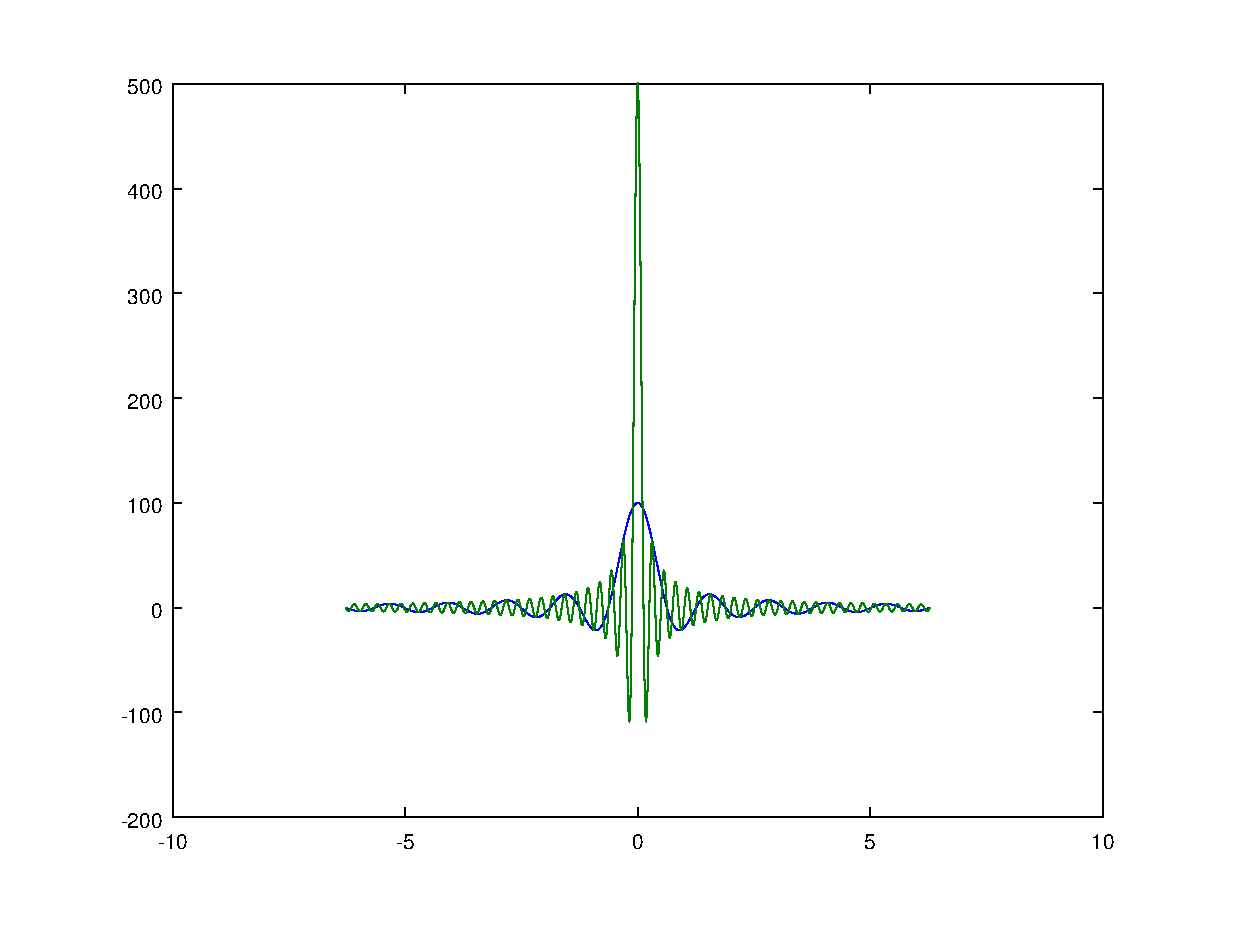
\includegraphics[width=0.8\textwidth]{1.eps}
\subsubsection{x:linear, y:log} 
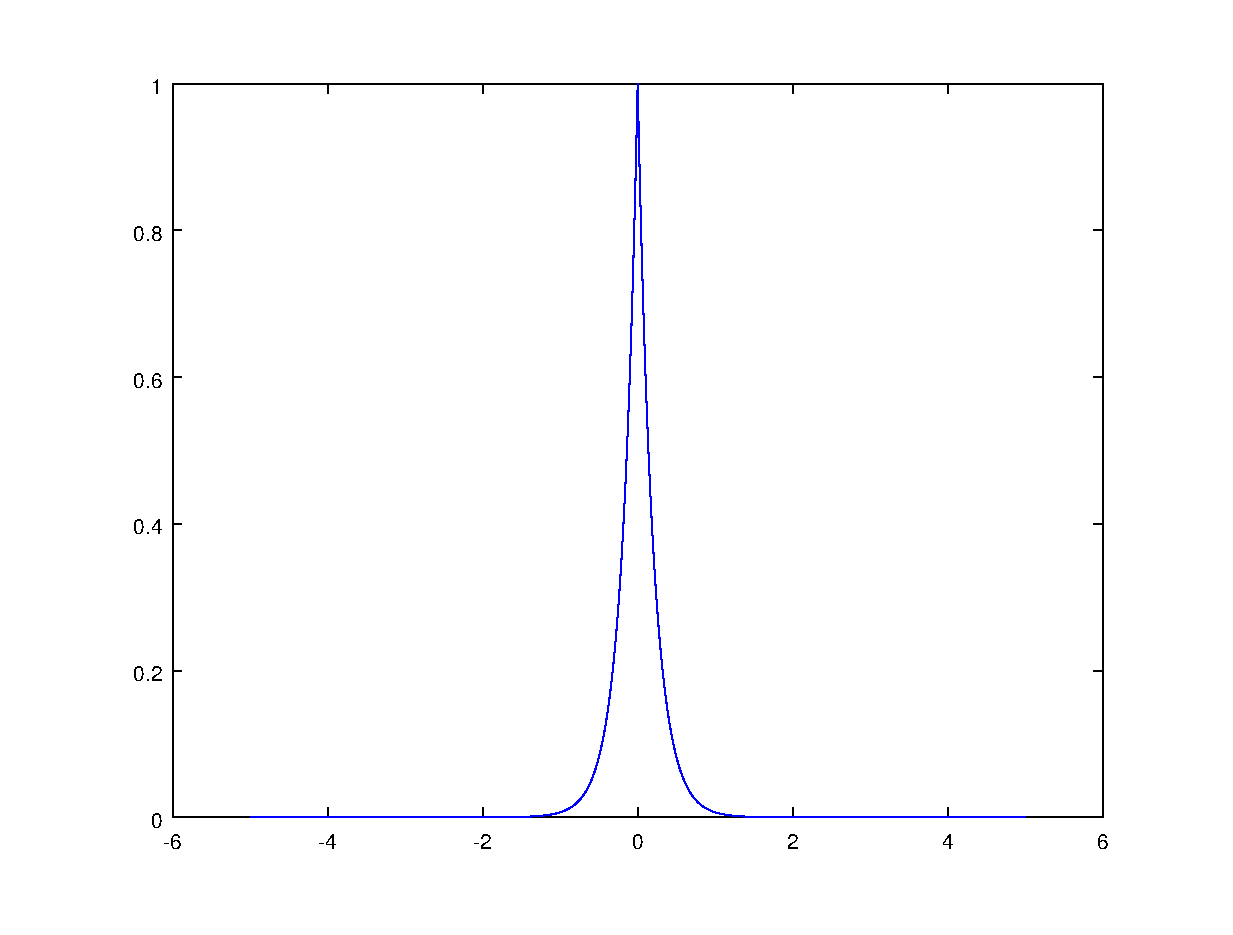
\includegraphics[width=0.8\textwidth]{2.eps}
\subsubsection{x:log, y:linear} 
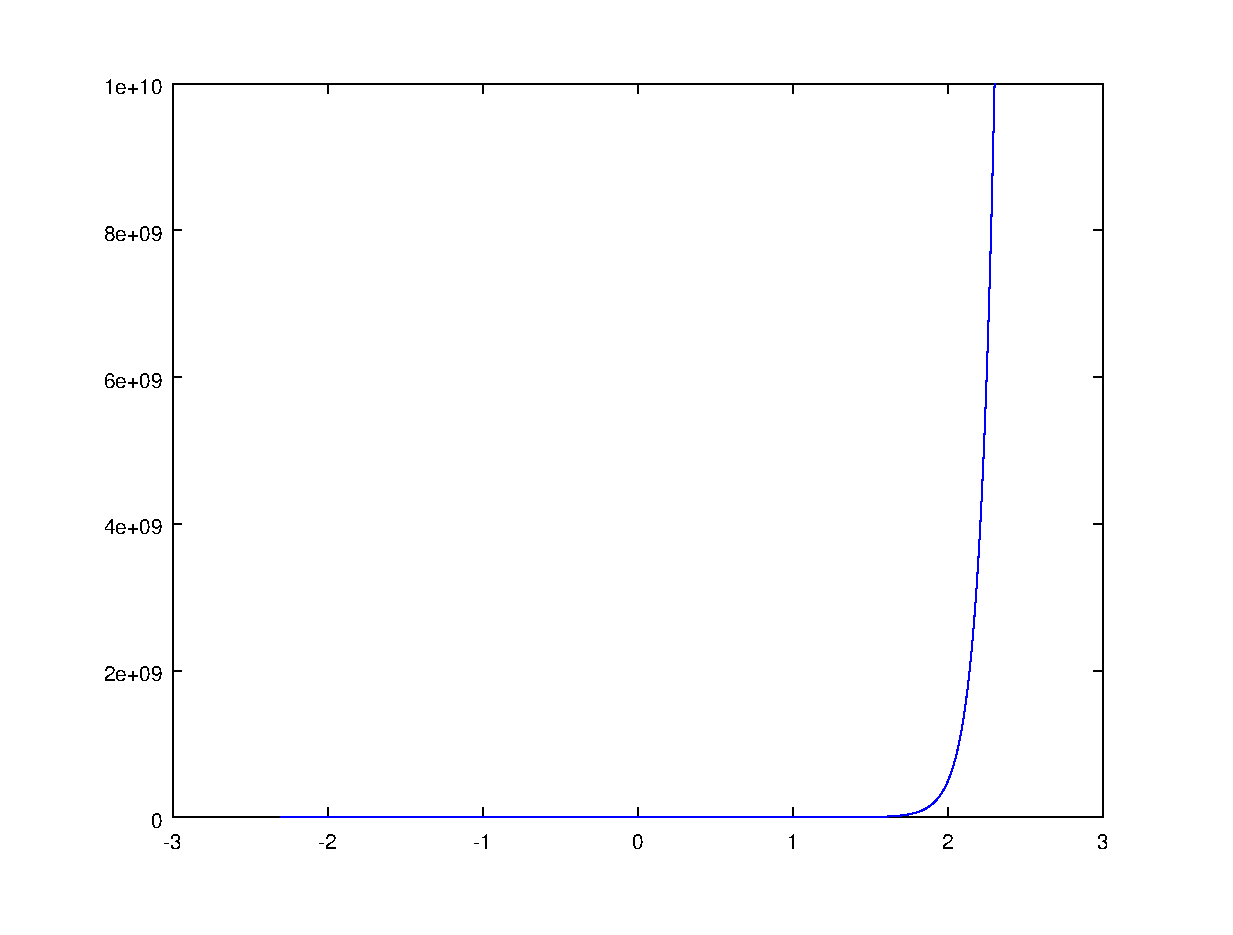
\includegraphics[width=0.8\textwidth]{3.eps}
\subsubsection{x:log, y:log} 
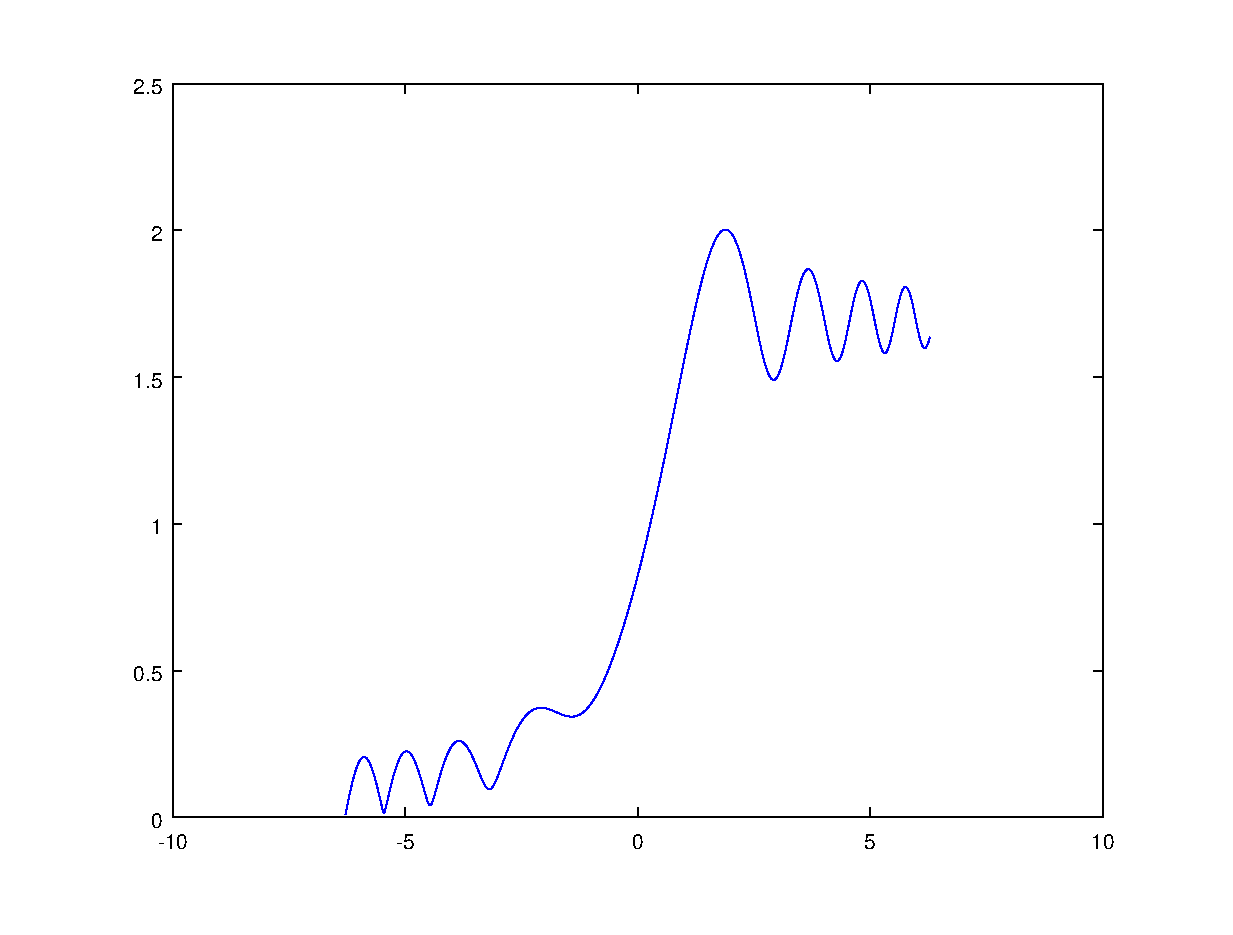
\includegraphics[width=0.8\textwidth]{4.eps}
\end{document}
